%%%% CAPÍTULO 2 - REVISÃO DA LITERATURA (OU REVISÃO BIBLIOGRÁFICA, ESTADO DA ARTE, ESTADO DO CONHECIMENTO)
%%
\chapter{Fundamentaç\~ao Te\'orica}\label{cap:fundamentacaoTeorica}

Este capítulo apresenta os conceitos relacionados a \gls{ca}. Primeiramente aborda-se a definição de \gls{ca}, seu uso em aplicações, os desafios enfrentados por essa estratégia e o detalhamento dos algoritmos de perforação de laço, memoização, aproximação de ponto flutuante e o descarte de tarefas. Apresenta também conceitos de Computação Paralela com um foco no uso da ferramenta OpenMP. Por fim, verificam-se trabalhos similares á presente pesquisa.

\section{Computação aproximada}\label{sec:compAprox}

A \gls{ca} consiste em um conjunto de técnicas aplicadas a cenários em que os resultados exatos não são estritamente necessários ou em que as aplicações apresentam resiliência suficiente para lidar com pequenas imprecisões em suas computações. Nessas situações, o uso de tais técnicas pode proporcionar ganhos significativos de desempenho e eficiência energética, mantendo a margem de erro em níveis reduzidos. Um exemplo é o uso de redes neurais para aproximar a divergência de \textit{branch} em instruções \gls{simd}, capaz de alcançar aceleração de até 14,8$\times$ com acurácia de 96\%~\cite{grigorian2015}. Por esse motivo, a \gls{ca} se mostra especialmente atraente em domínios como análise de dados, reconhecimento de padrões, processamento de imagens e sinais~\cite{mittal2016, chippa2013}.

As diferentes estratégias de aproximação podem ser classificadas conforme a camada em que são aplicadas na pilha computacional. No nível de \textit{hardware}, destacam-se técnicas que envolvem desde unidades funcionais aproximadas, como somadores, multiplicadores e divisores, até abordagens como \textit{overclocking}~\cite{leon2025a,leon2025b} e o uso de memórias aproximadas~\cite{fabricio2020}. No nível de \textit{software}, encontram-se estratégias mais generalistas, incluindo linguagens de programação aproximada~\cite{sampson2015}, \textit{runtimes} com suporte à aproximação~\cite{li2018,reis2024} e otimizações realizadas em nível de compilador~\cite{oliveira2024a,oliveira2024b}.

Apesar de seus benefícios, esse paradigma enfrenta desafios significativos. Em primeiro lugar, nem todas as aplicações são resilientes a erros em sua execução, o que limita o uso de técnicas mais generalistas e torna necessário definir métricas que permitam ajustar o grau de precisão desejado, seja pelo usuário ou pela própria aplicação~\cite{mittal2016}. Além disso, medir corretamente o nível de erro introduzido não é trivial, pois nem sempre está claro qual métrica deve ser aplicada à saída da aplicação~\cite{felzmann2021}. Outro ponto crítico é a propagação dos erros, que pode comprometer toda a execução: em alguns casos, a aplicação pode falhar abruptamente; em outros, concluir sua execução de forma aparentemente correta, mas com resultados significativamente distantes do esperado~\cite{fabricio2020}.

Diante disso é possível observar que a \gls{ca} não se restringe a um único método, mas a um conjunto de diversas estratégias que exploram diferentes aspectos da execução de um programa. Na subseção seguinte, são detalhados quatro dessas estratégias: perforação de laço, memoização, aproximação de ponto flutuante e o descarte de tarefas

\subsection{Perforação de laço}\label{subsec:perfLaco}

A perforação de laço é uma das técnicas mais simples de computação aproximada, cuja ideia central consiste em omitir determinadas iterações de um laço, reduzindo assim o tempo de execução de uma região de código~\cite{sidiroglou2011}.

Existem diferentes forma de implementar esse técnica, existem técnicas estáticas que são aplicadas em tempo de compilação e outras dinâmicas que permitem ajustar o grau de omissão em tempo de execução~\cite{li2018}.

Em ambos os casos é comum implementar essa otimização em laços que estão em um formato canônico~\cite{openmp2018}. A \autoref{code:loopCanon} apresenta a estrutura de um laço canônico, geralmente expresso na forma de um \texttt{for}, com três elementos principais:

\begin{itemize}
    \item \textbf{Expressão inicial:} define o limite inferior do laço, ou seja, o ponto em que a computação começa.
    \item \textbf{Expressão de teste:} geralmente um operador relacional que compara a variável de indução com o limite superior, delimitando o espaço de iterações.
    \item \textbf{Expressão de incremento/decremento:} atualiza a variável de indução e define o passo do laço.
\end{itemize}

\begin{sourcecode}[htb]\caption{\label{code:loopCanon}Estrutura de um laço canônico}
    \begin{lstlisting}[frame=single, language=C++]
        for (int i = 0; i < N; i += a) {
            ...
        }
    \end{lstlisting}
    \fonte{}
\end{sourcecode}

Uma técnica comumente encontrada na implementação desse algoritmo é a de incrementar a expressão de incremento, se considerarmos isso no \autoref{code:loopCanon} teríamos que a iterações deixariam de ser de \texttt{a} em \texttt{a} vezes, passaríamos a ter um incremento de \texttt{a + 1} vezes. Se considerarmos que inicialmente tem o valor \texttt{a = 1} ele passaria a ser \texttt{a = 2} e o comportamento do laço seguiria o que está na \autoref{fig:perfoMod}, nela temos que os blocos em branco seriam iterações não executadas enquanto os blocos em azul seriam iterações executadas.

Uma forma simples de aplicar a perforação de laço é alterar o passo do incremento da variável de indução, de modo que parte das iterações seja ignorada. No exemplo da \autoref{code:loopCanon}, se inicialmente o incremento for \texttt{a = 1} (\texttt{i++}), todas as iterações serão executadas. Entretanto, ao modificar o incremento para \texttt{a = 2} (\texttt{i += 2}), apenas metade delas será realizada, já que o laço passa a “pular” uma iteração a cada passo. Esse comportamento é ilustrado na \autoref{fig:perfoMod}, onde blocos em azul representam iterações executadas e blocos em branco representam iterações omitidas.

\begin{figure}[htb]
    \caption{Modelo de execução do algoritmo de perforação de laço}
    \label{fig:perfoMod}
    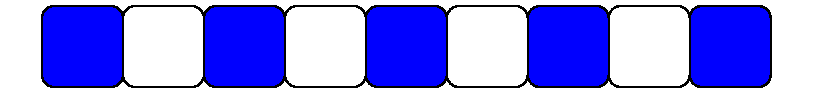
\includegraphics[scale=0.7]{Figuras/loop_perfo.pdf}
    \fonte{}
    \addcontentsline{loge}{figure}{\protect\numberline{\thefigure}Modelo de execução do algoritmo de perforação de laço.}
\end{figure}

\subsection{Memoização}\label{subsec:memo}

A memoização é tradicionalmente uma técnica associada à programação dinâmica que utiliza uma \textit{cache} de resultados para acelerar a execução de determinadas computações. Seu princípio consiste em armazenar os resultados de chamadas já realizadas, indexados pelas entradas correspondentes. Assim, quando a função é invocada novamente com os mesmos parâmetros, o valor previamente calculado é retornado diretamente, evitando a repetição da computação~\cite{michie1968}.

A memoização aproximada, também chamada de memoização temporal, estende esse conceito ao considerar tempo de execução e localização como critérios adicionais. Sua ideia principal é explorar o fato de que chamadas consecutivas a uma mesma função tendem a produzir resultados similares~\cite{tziantzioulis2018}.

Na prática, as saídas são armazenadas em uma estrutura de dados e reutilizadas seletivamente em chamadas subsequentes. As estratégias de \textit{cache} podem variar, incluindo modelos globais, específicos por função ou mesmo dependentes de contexto. O reuso é normalmente controlado por um limiar de tolerância, que avalia a variação das saídas: se os resultados permanecerem estáveis dentro desse limite, a função é considerada estável e, portanto, pode ser memoizada~\cite{tziantzioulis2018}.

\subsection{Aproximação de ponto flutuante}\label{subsec:pontoFlut}

A representação de números reais por meio de números de ponto flutuante envolvem aproximação por padrão devido a impossibilidade de representar valores contínuos, se torna impossível representar um número infinito com um número finito de \textit{bits}~\cite{monniaux2008}. Por esse motivo aritmética com números de ponto flutuante usualmente introduzem erros de aproximação que variam conforme a ordem de execução dessas operações, resultando em um valor completamente diferente do esperado. Um exemplo disso pode ser obervado na \autoref{fig:perfoMod}.

\begin{figure}[htb]
    \caption{Erro introduzido na aritmética de ponto flutuante.}
    \label{fig:floatPoint}
    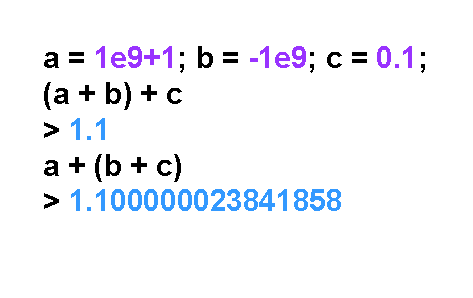
\includegraphics[scale=0.7]{Figuras/fastmath.pdf}
    \fonte{}
    \addcontentsline{loge}{figure}{\protect\numberline{\thefigure}Erro introduzido na aritmética de ponto flutuante.}
\end{figure}

Para reduzir este tipo de problema, compiladores usualmente evitam aplicar certas otimizações que podem amplificar o erro nesse tipo de operação. Porém, alguns compiladores como é o caso do \texttt{Clang} e o \texttt{GCC}, suportam a opção \texttt{--fast-math} que passa a permitir a aplicação dessas otimizações em todo um módulo de compilação~\cite{gccffast, clangffast}. E de maneira similar o \texttt{MSVC} suporta o uso da diretiva de compilação \texttt{\#pragma float\_control} para definir regiões do código que permitem o uso dessas otimizações em certas regiões decódigo~\cite{msvcfast}.

\subsection{Descarte de tarefas}\label{subsec:descTar}

O descarte de tarefas é um conceito abrangente que engloba diferentes técnicas de aproximação, incluindo, em alguns casos, a própria perforação de laço. Sua ideia central baseia-se em computações que podem ser divididas em unidades menores, chamadas tarefas, das quais uma parte delas é descartada~\cite{mittal2016}.

As implementações dessa técnica costumam adotar uma taxa de descarte, que define a fração de tarefas a serem eliminadas durante a execução do programa. A \autoref{fig:perfoMod} também pode ser utilizada para ilustrar esse mecanismo: os blocos brancos representam tarefas descartadas, enquanto os blocos azuis indicam as tarefas efetivamente executadas.

\section{Computação paralela}\label{sec:compParalela}

A computação paralela é uma área da computação que busca explorar arquiteturas modernas, cada vez mais baseadas em processadores \textit{multicore}. Esse conceito pode ser melhor compreendido a partir da taxonomia de Flynn~\cite{flynn1972}, que classifica as arquiteturas de computadores de acordo com o fluxo de instruções e de dados:

\begin{itemize}
    \item \textbf{SISD (\textit{Single Instruction, Single Data stream}):} Instrução única que atua sobre uma única fonte de dados.
    \item \textbf{SIMD (\textit{Single Instruction, Multiple Data stream}):} Instrução única que é aplicada simultaneamente a múltiplos dados.
    \item \textbf{MISD (\textit{Multiple Instructions, Single Data stream}):} Múltiplas instruções atuando sobre uma mesma fonte de dados.
    \item \textbf{MIMD (\textit{Multiple Instructions, Multiple Data stream}):} Múltiplas instruções atuando em paralelo sobre múltiplas fontes de dados.
\end{itemize}

Dentro desse modelo, o paralelismo pode ser explorado de diferentes maneiras. No nível do processador, técnicas como \textit{pipeline}, predição de desvios (\textit{branch prediction}) e escalonamento dinâmico permitem dividir o código em pequenas unidades que podem ser executadas simultaneamente.

Algumas arquiteturas foram além e incorporaram extensões \gls{simd}, permitindo a utilização de processadores vetoriais capazes de realizar a mesma operação sobre múltiplos elementos de um vetor unidimensional em um único ciclo de instrução. Em cenários mais especializados, como nas \glspl{gpu}, esse modelo é expandido para múltiplas dimensões de dados, possibilitando que milhares de operações sejam executadas em paralelo e tornando-as altamente adequadas para cargas de trabalho massivamente paralelizáveis~\cite{hennessy2017}. Outro mecanismo fundamental é o uso de \textit{threads}, que representam abstrações de execução em nível de software, permitindo que diferentes unidades computacionais operem concorrentemente em múltiplos processadores. Cada \textit{thread} possui seu próprio contexto de execução, mas pode compartilhar recursos como memória e dispositivos de entrada/saída, viabilizando desde o paralelismo de tarefas independentes até a cooperação em algoritmos que exploram granularidades mais finas~\cite{tanenbaum2015,hennessy2017}.

É nesse contexto que surge o OpenMP, uma \gls{api} projetada para estender C, C++ e Fortran com suporte à paralelização de aplicações por meio de anotações de código. Essas anotações especificam o como aquela região de código deve ser executada. Seu modelo de programação permite explorar automaticamente diferentes formas de paralelismo, seja pelo \textit{offloading} para \glspl{gpu}, pelo uso de múltiplas \textit{threads}, ou ainda pela vetorização via \gls{simd}, aproveitando as unidades vetoriais das arquiteturas modernas~\cite{mattson2019}.

O OpenMP é estruturado em uma arquitetura em camadas, composta por anotações de código, suporte da \textit{runtime} e configurações do ambiente de execução, conforme ilustrado na FIGURA. Esse modelo permite ao programador controlar diversos aspectos da execução por meio de diretivas e chamadas à biblioteca, como a definição do número de \textit{threads} em uma região paralela e a escolha do comportamento do escalonador. Dessa forma, o OpenMP oferece um controle flexível sobre o paralelismo do programa.

A \autoref{code:produtoVet} apresenta a implementação sequencial de um produto escalar entre vetores. A paralelização utilizando a biblioteca \texttt{pthreads}, apresentada no \autoref{code:produtoThread}, exige a criação explícita de \textit{threads}, gerenciamento de regiões de memória e sincronização dos resultados parciais. Em contraste, o ALGORITMO implementado com o OpenMP, evidencia a simplicidade proporcionada pelas diretivas: uma única anotação é suficiente para paralelizar o laço de cálculo, delegando à \textit{runtime} a criação e sincronização das \textit{threads}.

\begin{sourcecode}[htb]\caption{\label{code:produtoVet}Estrutura de um laço canônico}
    \begin{lstlisting}[frame=single, language=C++]
        for (int i = 0; i < N; i++) {
            result += a[i] * b[i];
        }
    \end{lstlisting}
    \fonte{}
\end{sourcecode}

\begin{sourcecode}[htb]\caption{\label{code:produtoThread}Estrutura de um laço canônico}
    \begin{lstlisting}[frame=single, language=C++]
        void *compute_partial_dot(void *arg) {
            ThreadArgs *args = (ThreadArgs *)arg;
            args->partial_sum = 0.0;
            
            for (int i = args->start; i < args->end; i++) {
                args->partial_sum = 0.0; += args->a[i] * args->b[i];
            }

            return NULL;
        }

    ...

    pthread_t threads[NUM_THREADS];
    ThreadArgs args[NUM_THREADS];
    result = 0.0;
    chunk_size = N / NUM_THREADS;

    for (int i = 0; i < NUM_THREADS; i++) {
        args[i].start = i * chunk_size;
        args[i].end = (i == NUM_THREADS - 1) ? N : (i + 1) * chunk_size;
        args[i].a = a;
        args[i].b = b;
        pthread_create(&threads[i], NULL, compute_partial_dot, &args[i]);
    }

    for (int i = 0; i < NUM_THREADS; i++) {
        pthread_join(threads[i], NULL);
        result += args[i].partial_sum;    
    }
    \end{lstlisting}
    \fonte{}
\end{sourcecode}

\begin{sourcecode}[htb]\caption{\label{code:loopCanon}Estrutura de um laço canônico}
    \begin{lstlisting}[frame=single, language=C++]
        #pragma omp parallel for reduction(+ : result)
        for (int i = 0; i < N; i++) {
            result += a[i] * b[i];
        }
    \end{lstlisting}
    \fonte{}
\end{sourcecode}

Tipicamente, uma diretiva OpenMP é aplicada a um laço para indicar que ele pode ser executado em paralelo. Durante a compilação, esse bloco de código é isolado e transformado em tarefas, enquanto a \textit{runtime} prepara as estruturas necessárias para o modelo \textit{fork-join}. Por exemplo, a diretiva \texttt{\#pragma omp parallel} cria um time de \textit{threads}, cada uma executando uma cópia do código anotado. O compilador gerencia variáveis privadas, memória de pilha e pontos de sincronização automaticamente. Ao final, as \textit{threads} são reunificadas (\textit{joined}), e a execução retorna ao fluxo sequencial. Essa abordagem permite paralelizar regiões de código com esforço reduzido de gerenciamento, mantendo controle sobre sincronização e compartilhamento de dados~\cite{mattson2019}.

O modelo \textit{fork-join} pode ser observado de forma esquemática na FIGURA. Nele, a \textit{runtime} cria múltiplas \textit{threads} para a execução paralela, que são sincronizadas ao final, restando apenas a \textit{thread} principal para continuar a execução sequencial. O OpenMP também suporta regiões paralelas aninhadas, possibilitando hierarquias de paralelismo.

\section{Trabalhos relacionados}\label{sec:trabRelac}

Ao longo dos anos uma grande variedade de \textit{frameworks} e metodologias vem sendo prosposta para suportar \gls{ca} em diferentes níveis de abstração. Os trabalhos apresentados nessa seção buscam prover técnicas em nível de \textit{runtime} e também buscam prover um equilibrío entre ganhos eficiência e qualidade de saída, usualmente utilizando estratégias de estatistíca, adaptação em tempo \textit{runtime} ou anotações em nível de linguagem de programação.

\texttt{ApproxHadoop}~\cite{goiri2015} é uma extensãoa ao \texttt{Hadoop} para suportar o descarte de seletivo tarefas (\textit{task dropping}) no \texttt{MapReduce}. Por meio de um mecanismo de amostragem dos dados de entrada, a extensão visa reduzir o tempo de execução e o consumo de recursos ao evitar o processamento completo dos dados, sem perder de vista a utilidade prática dos resultados. Além disso, o sistema integra métodos estatísticos que calculam limites de erro, fornecendo garantias quantitativas sobre a precisão das respostas aproximadas.

Rinard~\cite{rinard2006} propôs uma metodologia de particionamento da computação em tarefas que podem ser descartadas, seja em resposta a falhas ou de forma deliberada para melhorar o desempenho. Em sua abordagem a aplicação é decomposta em tarefas, que são analisdas para distinguir as essenciais daquelas que podem ser descartas, isso é feito por meio de um teste onde o programa é executado e a \textit{runtime} insere falhas de maneira proposital para verificar se o programa suporta aquela falha ou não, e também é usado um modelo de regrassão obtido por amostragem repetida para prever os efeitos dessas omissões.

Lashgar et al.~\cite{lashgar2018} propõem a integração da técnica de perforação de laço ao \texttt{OpenACC} com o objetivo de melhorar o desempenho, executando apenas um subconjunto das iterações do laço. Dessa forma, parte das saídas é calculada de maneira exata, enquanto o restante é aproximado. Para mitigar os impactos dessa abordagem na precisão e no tempo de execução dentro do \texttt{OpenACC}, os autores introduzem um mecanismo de correção implementado diretamente no kernel. Esse mecanismo identifica as saídas ausentes e aplica estratégias como a cópia ou a média dos valores vizinhos já computados, a fim de estimar as entradas faltantes.

O \texttt{Sculptor}~\cite{li2018} é um \textit{framework} geral para perforação de laço dinâmica e seletiva, que avança em relação às técnicas tradicionais ao permitir aproximações em nível fino, tanto no nível de instruções individuais quanto no nível das iterações. Diferentemente das abordagens clássicas, que pulam um subconjunto fixo de iterações de forma uniforme, o \texttt{Sculptor} seleciona dinamicamente quais instruções devem ser ignoradas dentro dos laços e ajusta, em tempo de execução, as taxas de perfuração e os pontos de início de acordo com o comportamento do programa. Ele emprega uma \textit{pipeline} de otimizações do compilador em múltiplas etapas, capaz de identificar instruções com baixo impacto na precisão, mas alto potencial de ganho de desempenho, transformando os laços de forma adequada. Além disso, o \textit{framework} inclui escalonadores dinâmicos que adaptam o grau de agressividade da perfuração entre diferentes contextos de chamada e fases do laço.

O \texttt{SampleMine}~\cite{jiang2022} é um \textit{framework} que acelera a mineração de padrões em subgrafos aplicando perforação de laço nos laços aninhados usados na exploração dos subgrafos. Ele introduz uma técnica de expansão baseada em dois vértices, na qual cada passo adiciona dois vértices ao subgrafo, reduzindo a complexidade computacional em comparação com os métodos tradicionais, que acrescentam apenas um vértice por iteração.

Vassiliadis et al.~\cite{vassiliadis2015} propõem um \textit{framework} que introduz um modelo de programação baseado em tarefas, no qual os desenvolvedores podem anotar cada tarefa com um nível de significância e, opcionalmente, fornecer versões aproximadas. A \textit{runtime} decide dinamicamente quais tarefas devem ser executadas de forma precisa ou aproximada, de acordo com as restrições de qualidade definidas pelo usuário. Duas políticas de execução são implementadas: \textit{Global Task Buffering (GTB)}, que armazena tarefas para permitir decisões globalmente informadas, e \textit{Local Queue History (LQH)}, que se baseia no histórico local das tarefas para decisões descentralizadas e mais rápidas.

\texttt{HPAC}~\cite{parasyris2021} é um \textit{framework} que integra suporte de compilador e de tempo de execução para habilitar computação aproximada em aplicações de \gls{hpc} utilizando OpenMP. Ele permite que os desenvolvedores anotem regiões de código com diretivas de aproximação e avaliem o equilibrío entre precisão e desempenho. O \texttt{HPAC} oferece suporte a técnicas como perforação de laço, memoização de entrada e saída, além de fornecer ferramentas para avaliar o impacto dessas técnicas na execução paralela.

\section{Considerações do capítulo}

Ao longo deste capítulo, foram apresentados os conceitos fundamentais de computação aproximada, alguma de suas principais técnicas. como perforação de laço, memoização, aproximação de ponto flutuante e descarte de tarefas, bem como noções de computação paralela com foco no OpenMP. Destacou-se que essas estratégias buscam melhorar desempenho e eficiência energética, mantendo resultados dentro de margens de erro aceitáveis, e que sua aplicação exige atenção às características das tarefas e ao contexto da execução. A revisão de trabalhos relacionados mostrou ainda como diferentes \textit{frameworks} implementam essas técnicas de forma dinâmica e adaptativa, fornecendo subsídios teóricos para os experimentos e metodologias apresentados nos capítulos seguintes.

